\documentclass[11pt]{article}
\usepackage{fullpage,graphicx,tabularx,amsfonts,
 bm,amsmath,bbm,extarrows}
 
%%%%%%%%%%% Biblio
\usepackage{natbib}
\bibliographystyle{unsrtnat}
\setcitestyle{authoryear}

\begin{document}
\title{\textbf{Natural Image Denoising with Deep Neural Networks}}
\author{Xuan Chen, Geng Ji, Shenglong Li, Zhonglei Wang}
\date{}
\maketitle
 
\section{Objective}
In this project, we aim to remove the additive white Gaussian noise from gray-scale natural images using end-to-end deep neural networks.

\section{Related work}
Natural image denoising is a well studied image processing task. 
Many non-deep-learning methods have reached success in this area.
The K-SVD method~\citep{elad2006image} generalizes K-means clustering to learn a dictionary for sparse coding of image patches.
The state-of-the-art \emph{learned simultaneous sparse coding} (LSSC)~\citep{mairal2009non} and \emph{block matching and 3D filtering} (BM3D)~\citep{dabov2008image} methods integrate clustering, dictionary learning, and denoising to extract information directly from a single corrupted image.
Alternatively, the \emph{expected patch log-likelihood}  (EPLL)~\citep{zoran2011learning} method maximizes the log-likelihood of overlapping image patches under a finite Gaussian mixture model learned from uncorrupted natural images.

A couple of deep neural networks have been developed for image denoising as well. 
\cite{jain2009natural} designed a four-layer convolutional neural network.
\cite{xie2012image} combined the idea of stacked denoising auto-encoders with sparse coding, and came up with a fully connected network called SSDA on image patches.
However, the performance of those methods are inferior the state-of-the-arts.
The reason might be that comparing to other tasks such as image classification where deep learning has already done pretty well, image denoising requires per-pixel intensity estimation so that the dimension of this problem is much higher than just predicting a single label.

\section{Our contributions}
\subsection{Short-term goals}
First, we hope to replicate the work done by \cite{jain2009natural} and \cite{xie2012image} using tensorflow.
The diagram for the CNN developed by \cite{jain2009natural} is shown in Fig.~\ref{fig:CNN}.
It takes in noisy images, and tries to minimize the mean square error against their Tuncorrupted counterparts.
The network contains four hidden layers, each with 24 feature maps that all share the same size with the input image.
Note that it is a pure CNN without any pooling layer which would otherwise shrink the size of the feature maps or any fully connected layer which would result in too many parameters to learn.
\begin{figure}
  \centerline{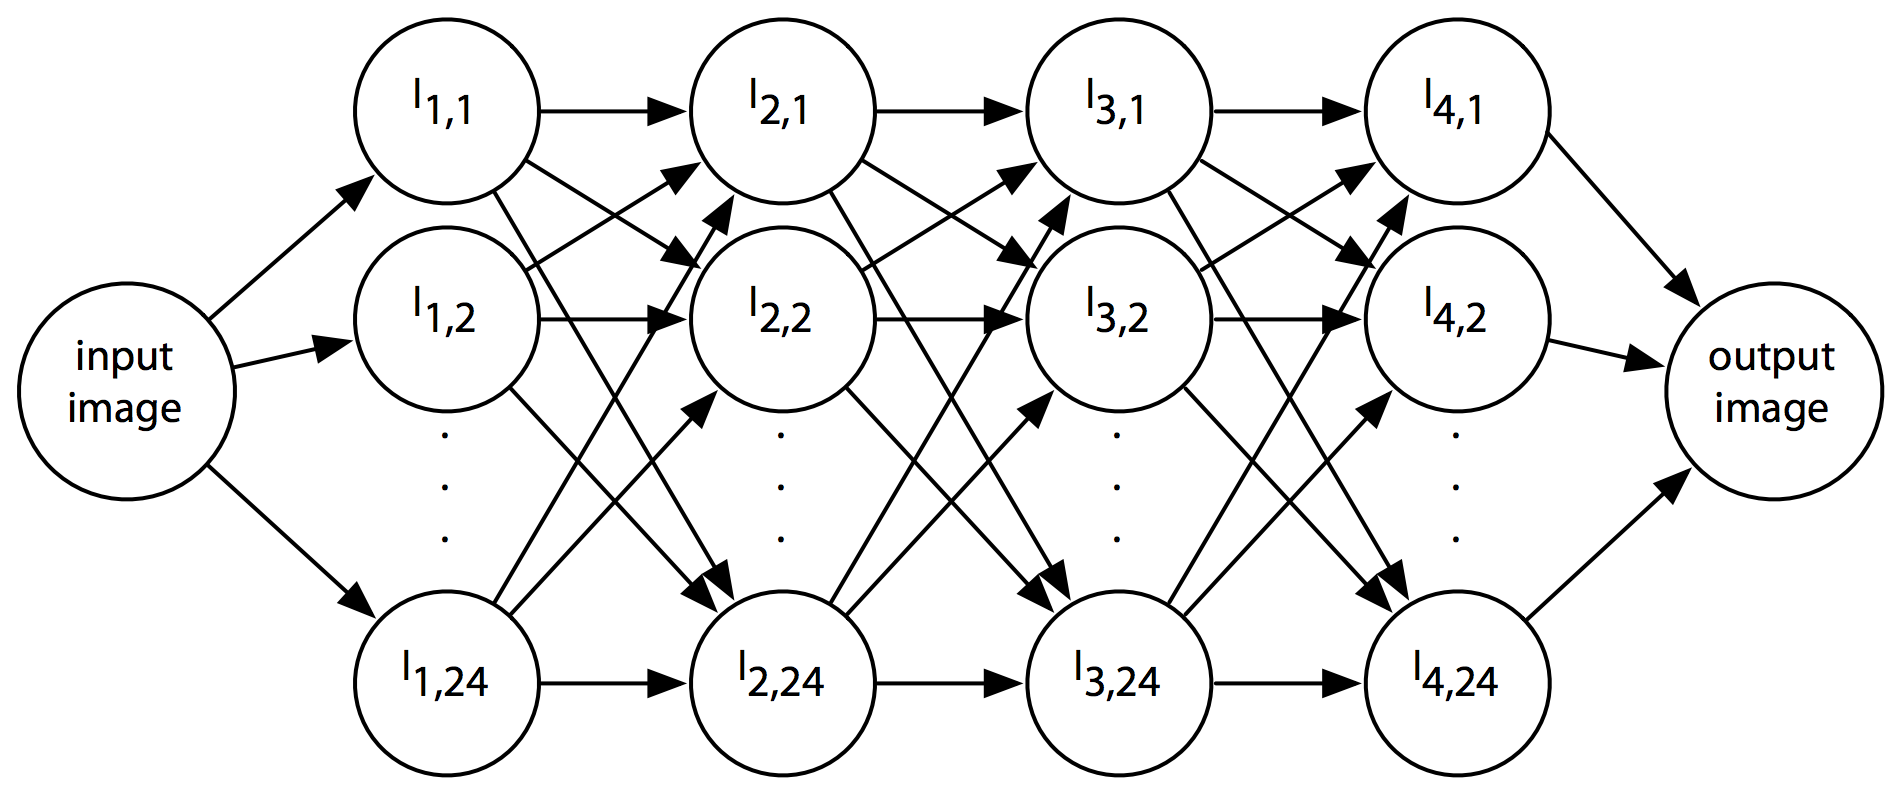
\includegraphics[width=2.5in]{CNN}}
  \caption{Convolutional neural network developed by \cite{jain2009natural}.}
  \label{fig:CNN}
\end{figure}

The sparse stacked denoising auto-encoders (SSDA) uses denoising auto-encoders (DA) as building blocks, a popular pre-training framework, and stacks up four layers of them, as shown in Fig.~\ref{fig:SSDA}.
For each DA, it tries to learn a pair of weights $W$ that encodes the noisy input $x=\eta(y)$ and $W'$ that decodes it into the clean counterpart $y$.
To enhance sparsity, the loss function $L(x,y)$ contains not only the mean square error between $x$ and $y$, but also some regularization terms for the weight parameters in the network.

\begin{figure}
  \centerline{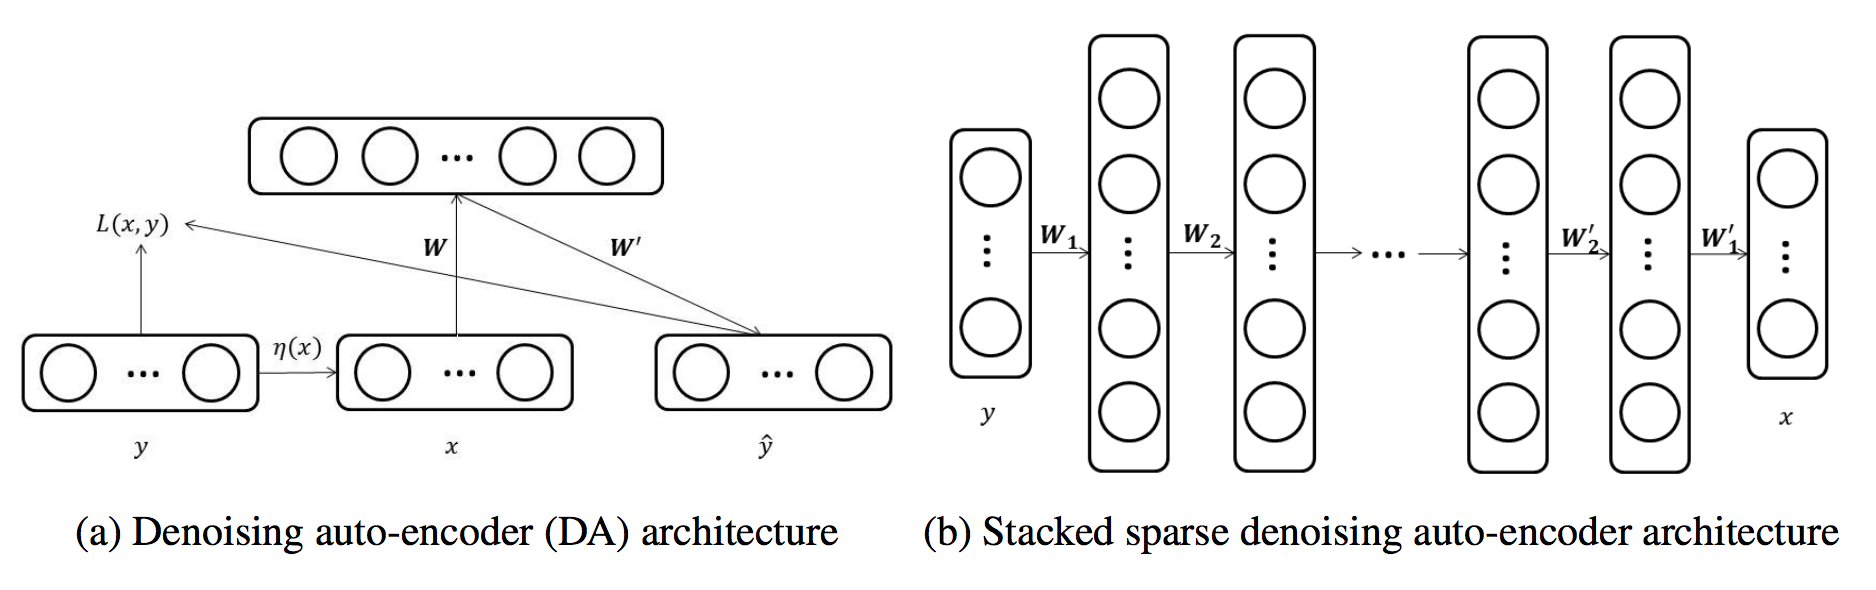
\includegraphics[width=3.5in]{SSDA}}
  \caption{Sparse stacked denoising auto-encoder developed by \cite{xie2012image}.}
  \label{fig:SSDA}
\end{figure}


\subsection{Long-term goals}
Our long-term goal is to improve the two networks for better performance.
For example, we may add more layers to each of them, and make use of dropout to prevent overfitting.
If time allows, we also plan to try other types of recently developed networks such as ResNet and Highway networks.

\section{Dataset Link}
We use the Berkeley Segmentation Dataset for both training (400 images) and test (100 image). 
Its link is https://www2.eecs.berkeley.edu/Research/Projects/CS/vision/bsds/.
We've already started training the networks shown in Fig.~\ref{fig:CNN} and Fig.~\ref{fig:SSDA} on this dataset using our machines, but it takes too much time.
We've talked to the TA's about using the GPU version of tensorflow on department machines and got positive feedback. 
Hopefully packages like scipy could be correctly installed on those machines in a short time so that we may run our code there.

{\small
\linespread{1}
\bibliography{REFERENCE}
}

\end{document}